\documentclass[a4paper, 12pt, titlepage, finall]{extreport}

%различные пакеты

\usepackage[T1, T2A]{fontenc}
\usepackage[russian]{babel}
\usepackage[backend=bibtex]{biblatex}
%\usepackage{booktabs}
\usepackage{tikz}
\usepackage{geometry}
\usepackage{indentfirst}
\usepackage{fontspec}
\usepackage{graphicx}
\usepackage{array}
\graphicspath{{./images/}}
\renewcommand{\baselinestretch}{1.25}
\usetikzlibrary{positioning, arrows}

%\geometry{a4paper, left = 15mm, top = 10mm, bottom = 20mm, right = 15mm}
\geometry{a4paper, left=1.18in, top=0.79in, bottom=0.79in, right=0.59in}

\setmainfont{Spectral Light}%{Times New Roman}
\setmonofont{Noto Sans}
%\setcounter{secnumdepth}{3}
%\setcounter{tocdepth}{3}

\bibliography{vqr} 

\begin{document}

    \begin{titlepage}
        \begin{center}
            {\small \sc Московский государственный университет имени М.~В.~Ломоносова\\
            Факультет вычислительной математики и кибернетики\\
            Кафедра автоматизации систем вычислительных комплексов\\}
            \vfill
            {\large \sc Выпускная квалификационная работа}\\~\\

            {\large \bf Исследование применимости алгоритмов сжатия данных к таблицам классификации в сетевом процессорном устройстве}\\~\\

        \end{center}
        
        \begin{flushright}
            \vfill
            \vfill
            {Никифоров Никита Игоревич, 421 группа}\\
            {Научные руководитель:}\\
            {к. ф.-м. н., доцент Волканов Д. Ю.,}\\
        \end{flushright}

        \begin{center}
            \vfill
            {\small Москва\\2021}
        \end{center}
    \end{titlepage}

    \chapter*{Аннотация}
        В данной работе рассматривается архитектура сетевого процессорного устройства (СПУ), в которой используется конвейерная архитектура.
        Конвейер состоит из последовательных вычислительных блоков, в каждом из которых находится независимое устройство памяти.
        В памяти вычислительного блока хранится программа классификации пакетов.         

    \newpage
    \tableofcontents
    \newpage

    \chapter*{Введение}
        \addcontentsline{toc}{chapter}{\protect\numberline{}Введение}%
        В настоящее время активно развиваются технологии программно-конфигурируемых сетей (ПКС). Для работы ПКС требуются высокопроизводительные коммутаторы, 
        которые выполняют функцию передачи данных. Возникает задача разработки программируемого сетевого процессорного устройства (СПУ),
        являющегося основным функциональным элементом коммутаторов. В работе рассматривается коммутатор функционирующих под управлением протокола OpenFlow.
        Правила обработки пакетов в котором представляются в виде таблицы потоков. В данной работе рассматриваются только простые таблицы потоков.
        В СПУ таблицы потоков представляются в виде программы обработки заголовков сетевых пакетов.


        СПУ представляет из себя интегральную микросхему. В рассматриваемом СПУ применяется конвейерная архитектура,
        а именно на каждый входной порт коммутатора СПУ содержит конвейер, состоящий из вычислительных блоков. Каждый вычислительный блок имеет доступ к 
        устройству памяти в котором хранится программа обработки заголовков сетевых пакетов. Рассматриваемый СПУ имеет ограниченный объём доступной
        памяти, для хранения программы обработки заголовков сетевых пакетов.

        Современные таблицы потоков занимают до нескольких десятков мегабайтов памяти \cite{rottenstreich2016optimal}. Поэтому возникает задача сжатия таблиц потоков,
        для использования рассматриваемого СПУ в коммутаторах ПКС.


    \chapter{Цели и задачи работы}
        Целью данной работы является исследование и разработка алгоритмов сжатия данных для применения к таблицам потоков OpenFlow. Для достижения поставленной цели
        необходимо было выполнить следующие задачи:
        \begin{itemize}
            \item Провести обзор существующих алгоритмов сжатия данных и способов их применения для сжатия таблиц потоков OpenFlow с целью выбора 
                для применения в рассматриваемой архитектуре сетевого процессорного устройства.
            \item Провести анализ изменений, необходимых для применения в данном сетевом процессорном устройстве.
            \item Внести необходимые изменения в выбранные алгоритмы сжатия данных.
            \item Реализовать выбранные алгоритмы сжатия данных для проверки на эмуляторе сетевого процессорного устройства.
            \item Реализовать необходимые изменения эмулятора сетевого процессорного устройства, необходимые для проверки реализованных алгоритмов
                сжатия данных.
            \item Провести экспериментальное исследование реализованных алгоритмов сжатия данных.
        \end{itemize}
    \chapter{Рассматриваемая архитектура сетевого процессора}
        \label{chapt:arch}
        В рамках работы важны лишь некоторые особенности рассматриваемой архитектуры, а именно, отсутствие выделенного ассоциативного устройства памяти и конвейерная архитектура. 
        Данные особенности непосредственно влияют на ограничения, предъявляемые к реализуемым структурам данных.

        В сетевом процессоре используется конвейерная архитектура, каждый конвейер состоит из 10 вычислительных блоков. 
        Вычислительный блок $-$ это набор более низкоуровневых RISC ядер, которые в данной работе не рассматриваются. 
        Каждый вычислительный блок имеет доступ к участку памяти, в котором располагаются микрокод и данные.
        Существует ограничение на количество тактов, которое один пакет может обрабатываться на вычислительном блоке, оно соответствует 25 тактам.
        Данное ограничение обусловлено требованием к производительности сетевого процессора, а именно фиксированное время обработки одного пакета на сетевом процессоре.
        Также один вычислительный блок имеет доступ к 64 килобайтам памяти.
        Из-за особенностей микроархитектуры, отсутствует отдельная область памяти, в которой хранятся данные. Поэтому микрокод содержит в себе все данные,
        необходимые для классификации пакетов.

        \begin{figure}[h]
            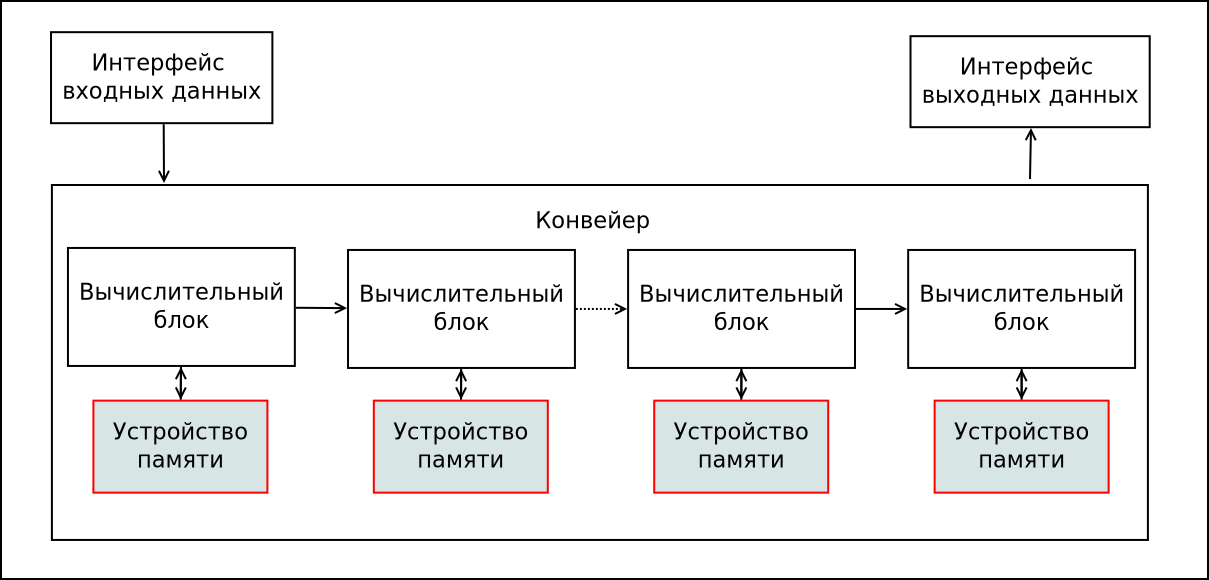
\includegraphics[width=\textwidth]{npu_all.png}
            \caption{Архитектура рассматриваемого сетевого процессора}
        \end{figure}
        
    \chapter{Постановка задачи} 
    \section{Не формальная постановка задачи}
        Необходимо исследовать применимость существующих алгоритмов сжатия данных в существующей архитектуре СПУ.
        Рассматриваемые алгоритмы должны удовлетворять следующим условиям:
        \begin{itemize}
            \item Размер итоговой таблицы потоков не должен превышать 512 Кб.
            \item Потери данных при использования алгоритмов сжатия не должны быть значительными.
            \item Сжатую таблицу потоков должно быть возможно использовать без декомпрессии.
        \end{itemize}

    \section{Формальная постановка задачи}
        \label{sect:problem}
        Введём формализацию OpenFlow таблиц.
        Упорядоченное множество всех рассматриваемых признаков в правилах обозначим \(I=\{m_1,m_2,\ldots,m_k\}\). 
        Каждый признак \(m_i\) из множества признаков \(I\) характеризуется битовой строкой, некоторой длины \(m_i \in \{0, 1, *\}^W_i\),
        в данном случае символ \(*\) обозначает любой бит. При этом, если \(\exists m_i^j \in m_i\), такое, что 
        \( m_i^j = *\), то для \( \forall m_i^k \), где \(k > j\), то \( m_i^k = *\). Длиной признака обозначим \(len(m_i) = W_i\)

        Представим таблицу потоков в виде множества правил \(R=\{r_1,r_2,\ldots,r_n\}\). С каждым правилом \(r_i\) связаны:
        \begin{itemize}
            \item номер \(i\);
            \item приоритет \(p_i\in \mathbb{Z}_+\);
            \item вектор значений признаков \(f_i=\{f_i^1,f_i^2,\ldots,f_i^k\}\), где \(f_i^j\) соответствует значению признака \(m_j\in I\). % и \(f_i^j\in D(m_j)\cup\{*\}\), \(j=\overline{1,k}\).
            \item Набор действий, \(A_i = \{a_1, a_2, \ldots, a_z\} \), которые определяют дальнейшие действия сетевого процессора над пакетом.
        \end{itemize}

        Будем говорить, что заголовок пакета \(x\) и его метаданные с вектором значений признаков \(g=\{g^1,g^2,\ldots,g^k\}\) (далее \(x \rightarrow g\)),
        соответствуют правилу \(r_i\in R\) с вектором значений признаков \(f_i=\{f_i^1,f_i^2,\ldots,f_i^k\}\) 
        и приоритетом \(p_i\) (правило \(r_i\in R\) идентифицирует пакет с вектором значений признаков \(g\)), если:

        \begin{enumerate}
            \item вектор значений признаков \(g\) соответствует вектору значений признаков \(f_i\), 
                то есть \(\forall g_i \in g\), \(len(g_i) = len(f_i)\). И \(\forall f_i^{lj} \in f_i^l\), \(f_i^{lj} \in \{*, g^{lj}\}\), \(l=\overline{1,k}\);
            \item приоритет \(p_i\) максимален среди всех правил \(r_j\in R\), для которых \(g\) соответствует вектору значений признаков \(f_j\).
        \end{enumerate}

        Множество \(R\) также должно удовлетворять следующему ограничению. 
        Для любых двух правил \(r_i,r_j\in R,r_i\not= r_j\), если их вектора значений пересекаются, то есть существует набор значений признаков, 
        который соответствует векторам значений признаков обоих правил, то \(p_i\not= p_j\). 
        Например, правила с векторами значений признаков \(f_i=\{110, 011, 1*\}\) и \(f_j=\{11*, 011, 11\}\) должны иметь разный приоритет, 
        так как набор значений признаков \(g=\{110, 011, 11\}\) соответствует обоим правилам.
        
        Введём функцию идентификации заголовка пакета \(x \rightarrow g\) в таблице потоков \(R\) и обозначим её \(R(x)\).
        Функция идентификации заголовка возвращает набор действий, соответствующий правилу, идентифицирующему заголовок пакета \(x \rightarrow g\).
        Таким образом \(R(x) = A_{r_i}\), где \(A_{r_i}\) набор действий правила \(r_i \in R\).

        Введём понятие аналогичности множеств \(R_1\) и \(R_2\).
        Множество \(R_1\) аналогично множеству \(R_2\), если для любого заголовка пакета, для которого существует идентифицирующее его правило \(r_i \in R_1\), 
        найдётся правило идентифицирующее его в множестве \(r_j \in R_2\), при этом \(A_i = A_j\).

        Необходимо разработать алгоритм сжатия таблиц потоков, который будет переводить исходное множество $-$ \(R_1\), соответствующее исходной таблице потоков, в
        новое множество \(R_2\), которое соответствует новой таблице потоков.
        \begin{enumerate}
            \item Множество \(R_1\) должно быть аналогично множеству \(R_2\).
            \item Мощность множества \(R_2\) должна быть меньше либо равно мощности множества \(R_1\).
        \end{enumerate}

        Введём операцию последнего значащего бита признака \(last(m_i) = j\), такое, что \(m_i^j \in \{0, 1\}\) и \(m_i^{(j+1)} = *\). 
        Назовём правила \(r_i \in R\) и \(r_j \in R\) похожими, 
        если для \(\forall u \in len(f_i)\) верно, что \(last(f_i^u) = last(f_j^u) = l\), при этом \(f_i^{ul} \neq f_j^{ul}\), и \(A_i = A_j\).



    \chapter{Обзор существующих алгоритмов сжатия}
        \section{Цель и задачи обзора}
        Целью данного обзора является выбор алгоритмов сжатия для применения в сетевом процессорном устройстве. 
        Необходимость применения алгоритмов сжатия обусловлена недостатком объёма памяти конвейера сетевого процессорного устройства.
        
        В настоящем обзоре будут использоваться следующие критерии:
        \begin{enumerate}
            \item Отношение объёма памяти занимаемого таблицей классификации после применения алгоритма сжатия, 
                к изначальному объёму памяти занимаемому таблицей классификации (Степень сжатия).
            \item Оценка сложности сжатия.
            \item Возможность использования без декомпрессии таблиц классификации $-$ 
                из-за ограничений рассматриваемого сетевого процессорного устройства сжатые таблицы классификации 
                должны представляться как код ассемблера.
            \item Использование внешней памяти $-$ необходимость использования внешней памяти 
                для использования сжатых таблиц классификации без декомпрессии.
        \end{enumerate}

        Данные критерии обусловлены особенностями рассматриваемой архитектуры СПУ. 
        Критерий \textbf{степень сжатия} необходим для оценки эффективности работы алгоритма сжатия.
        Критерий \textbf{оценки сложности сжатия} необходим для оценки накладных расходов на центральный процессор коммутатора при использовании рассматриваемого
        алгоритма сжатия.
        Критерий \textbf{возможности использования сжатых таблиц потоков без декомпрессии} обусловлен ограничениями архитектуры СПУ, а именно
        отсутствием адресуемой памяти в вычислительных блоках конвейера и ограниченным набором команд доступных СПУ (Раздел ~\ref{chapt:arch}).
        Критерий \textbf{необходимости использования внешней памяти} обусловлен дополнительными накладными расходами при обработке сетевым процессорным устройством 
        заголовков сетевых пакетов.

        Для описания алгоритмов сжатия в обзоре будет использована терминология описанная в разделе~\ref{sect:problem}. 

    \section{Рассматриваемые алгоритмы сжатия}
        \subsection{Распространённые алгоритмы}
            Под распространёнными алгоритмами сжатия будем понимать алгоритмы, 
            которые сжатые данные представляют в бинарном виде~\cite{kodituwakku2010comparison}. 
            Примером таких алгоритмов может служить:
            \begin{itemize}
                \item алгоритм Хаффмана,
                \item JPEG,
                \item LWZ,
                \item zip.
            \end{itemize}
            
            Рассмотрим критерии для данного класса алгоритмов. Различные алгоритмы в данной группе имеют различную \textbf{степень сжатия}, 
            которая колеблется от 0.3 до 0.8. Большинство рассматриваемых алгоритмов имеют квадратичную или кубическую \textbf{сложность сжатия} 
            от объёма сжимаемых данных. Так как сжатые данные после применения алгоритмов из данной группы представляются в бинарном виде,
            \textbf{невозможно использовать сжатые таблицы классификации без декомпрессии}. И некоторые алгоритмы из рассматриваемой группы требуют доступ к \textbf{внешней памяти}.
        \subsection{Алгоритм оптимального кеширования}
            Данный алгоритм основан на построение дерева поиска правил относительно их частот~\cite{rottenstreich2016optimal}, при этом, в данное дерево
            попадают только правила с определёнными частотами использования (далее популярность). 
            Правила, не попавшие в основное дерево, хранятся на центральном процессоре коммутатора и  доступ к ним осуществляется по запросу СПУ.
            
            Для описания данного алгоритма потребуется ввести дополнительные обозначения. Введём понятие распределения заголовков пакетов \(P\),
            где \(p_x\) обозначает вероятность получения пакета \(x \rightarrow g=\{g^1,g^2,\ldots,g^k\}\).
            Также введём понятие коэффициента правильности \(T_P(R_1, R_2)\), где \(R_1\) и \(R_2\) две различные таблицы потоков. 
            Таким образом коэффициент правильности обозначает вероятность того, что заголовок пакета, согласно распределению \(P\),
            будет в идентифицироваться правилами \(r_1 \in R_1\) и \(r_2 \in R_2\) и их наборы действий совпадают \(A_1 = A_2, A_1 \in r_1, A_2 \in r_2\).
            
            \[T_P(R_1, R_2) = \sum_{x \rightarrow g, R_1(x) = R_2(x)} p_x\]

            Введём оптимальное значение коэффициента правильности для заданной таблицы потоков \(R\), числа правил \(n\) и распределения заголовков \(P\).
            \[\zeta(n, R, P) = \max_{R_i, |R_i| <= n} T_P(R, R_i)\]
            
            Таким образом алгоритму необходимо найти и построить таблицу потоков \(R_a\), основанную на данной таблице потоков \(R\)
            с наименьшим количеством правил \(n_0\) и максимальные оптимальным коэффициентом правильности \(\zeta(n, R, P)\).
            Пусть \(p^i\) популярность (вероятность) выбора правила \(r_i \in R\), в соответствие с распределением заголовков \(P\). Пусть
            правила в таблице потоков \(R\) расположены в порядке не возрастания их популярности. Тогда:
            \[\zeta(n, R, P) \geq \sum_{i \in [1, n]} p^i + 1 - \sum_{i \in [1, n_0]} p^i \geq n/n_0\]

            Рассмотрим критерии для данного алгоритма: \textbf{Степень сжатия} данного алгоритма зависит от распределения частот использования префиксов, от 0.1 до 0.9.
            Данный алгоритм имеет квадратичную \textbf{сложность построения}. Сжатые таблицы классификации \textbf{возможно использовать без декомпрессии}.
            Для работы данного алгоритма \textbf{требуется внешняя память}, так как часть префиксов, которая не попала в выборку наиболее часто используемых хранится в
            памяти центрального процессора коммутатора.
        \subsection{Алгоритм Recursive endpoint cutting}
            Данный алгоритм основан на применении дерева HyperSplit, а сжатие производится за счёт удаления дублирующихся правил.~\cite{chang2019fast}
            Данный алгоритм поддерживает добавление и удаление правил в таблице потоков.

            Под дублирующимися правилами в таблице потоков понимаются следующие правила:
            \begin{itemize}
                \item правило, содержащиеся в вершине дублируется правилом в вершине, являющийся листом для данной вершины (частично дублирующиеся правило);
                \item правило, содержащиеся в вершине дублируется правилами во всех вершинах, являющихся листьями для данной вершины (полностью дублирующиеся правило).
            \end{itemize}
            Соответственно дублирующиеся правила перемещаются наверх дерева, что позволяет удалить полностью дублирующиеся правила.
            
            Рассмотрим критерии для данного алгоритма: \textbf{Степень сжатия} данного алгоритма приблизительно равна 0.15.
            Данный алгоритм имеет \textbf{сложность построения} \(n*log(n)\). Сжатые таблицы классификации \textbf{возможно использовать без декомпрессии}.
            Для работы данного алгоритма \textbf{не требуется внешняя память}, так как всё сжатие происходит в момент трансляции таблицы потоков в
            программу на языке ассемблера.
        \subsection{Алгоритм с использованием битовых векторов для представления таблиц потоков}
            Данный алгоритм основан на применение битовых строк для представления таблиц потоков. А именно таблица потоков разбивается на несколько частей,
            в каждой из которых для всех битов префиксов записывается два значения: подходит ли данный префикс, если в искомой строке 1, 
            подходит ли данный префикс, если в искомой строке 0. Таким образом поиск по таблицам потоков будет состоять из последовательного применения 
            операции and.

            Рассмотрим критерии для данного алгоритма: \textbf{Степень сжатия} данного алгоритма равна 0.5.
            Данный алгоритм имеет квадратичную \textbf{сложность построения}. Сжатые таблицы классификации \textbf{возможно использовать без декомпрессии}.
            Для работы данного алгоритма \textbf{требуется внешняя память}.
            %\subsection{Укороченное КД-дерево}
        %   Данный алгоритм основан на построение обычного КД-дерева. Разберём простой алгоритм построения КД-дерева:
        %   \begin{itemize}
        %    \end{itemize}
        \section{Сравнение алгоритмов сжатия}

        \section{Выводы}    
    \chapter{Эмулятор сетевого процессора}
        Эмулятор сетевого процессора $-$ программа написанная на языке программирования $python3$, которая позволяет эмулировать работу сетевого процессора, 
        а именно получать пакеты на любой из 24-х портов, обрабатывать пакет, получая информацию о любой стадии обработки, и отправлять пакет на выходные порты.
        Эмулятор сетевого процессора позволяет оценить количество тактов затраченных на обработку пакета, а также объём памяти затраченный на структуру данных.

        \section{Описание программных средств эмулятора сетевого процессора}
            Передача пакетов на порты сетевого процессора осуществляется с помощью файлов $.pcap$, в которых можно описать поступление пакетов на каждый порт в определённые моменты времени.
            В данной работе, не уменьшая общности, будет рассматриваться только один порт эмулятора сетевого процессора. Так как для каждого входного
            порта используется соответствующий конвейер. Изначально, в конвейере эмулятора сетевого процессора был реализован один вычислительный блок.
            Для проведения экспериментального исследования в данной работе, необходимо внести изменения в эмулятор сетевого процессора, а именно увеличить количество вычислительных блоков 
            в конвейере до 10.
        \section{Программные средства разработанные для проведения экспериментального исследования}
            Для проведения экспериментального исследования в рамках данной работы, необходимо разработать генератор сетевого трафика, который должен удовлетворять следующим требованиям:
            \begin{itemize}
                \item Возможность генерации L2 и L3 трафика.
                \item Возможность использовать наперёд заданную базу префиксов или mac-адресов для генерации трафика.
                \item Возможность использовать для генерации трафика заданное количество случайных префиксов или mac-адресов.
                \item Возможность сохранить базу использованных префиксов или mac-адресов.
                \item Возможность задать распределения времени поступления пакетов.
            \end{itemize}
            Для реализации будет использовать язык программирования $python3$, так как существует открытая библиотека $scapy$, которая позволяет работать с L2 и L3 трафиком,
            а так же позволяет сохранять сгенерированные пакеты в $.pcap$ файлы, что необходимо, для дальнейшего использования в эмуляторе сетевого процессора.
    \chapter{Система трансляции таблиц потоков в язык ассемблера сетевого процессорного устройства}
        В данной главе приводится описание системы трансляции таблиц потоков OpenFlow~\ref{mark}. Также будет представлено описание
        структур данных, использующихся для промежуточного представления таблиц потоков, и разработанных алгоритмов сжатия таблиц потоков и трансляции
        сжатых таблиц потоков в язык ассемблера СПУ.
        \section {Структуры данных}
            \subsection {Структура данных для представления таблиц потоков в виде дерева}
                В системе трансляции для представлении таблицы потоков с набором правил \(R\) используется дерево с помеченными вершинами и дугами.
                С каждой вершиной дерева, кроме вершин-листьев, связаны следующие значения:
                \begin{itemize}
                    \item признак из множества рассматриваемых признаков;
                    \item подмножество набора правил R.
                \end{itemize}

                Структура данных строится по следующим правилам, где \(v\) $-$ вершина дерева, которой соответствует признак \(m\) и подмножество правил \(S \subset R\):
                \begin{enumerate}
                    \item корню дерева соответствует всё множество правил \(R\);
                    \item если \(M\) $-$ множество всевозможных значений признака \(m\) в правилах из подмножества \(S\), то для каждого значения \(f \in M\)
                        у вершины \(v\) существует потомок, к которому ведёт дуга с пометкой \(f\).
                    \item если вершины \(u\) $-$ потомок вершины \(v\) в которую ведёт дуга с пометкой \(f\), то подмножество правил вершины \(u\) состоит только из
                        правил в \(S\), у которых значение признака \(m\) равно \(f\).
                \end{enumerate}

                Описанная структура данных позволяет выполнять поиск идентифицирующего обрабатываемый пакет правила в таблице потоков.
            \subsection{Структура данных для представления таблиц потоков в виде АВЛ дерева}
                В прошлой работе~\ref{nik_avl} была разработана структура данных для представления таблиц классификации в виде АВЛ дерева.
                Аналогично таблицу потоков можно также представить в виде АВЛ дерева, с каждой вершиной АВЛ дерева связаны следующие значения:
                \begin{itemize}
                    \item скалярное значение соответствующее набору признаков \(I = {m_1, m_2, \ldots, m_k}\), вычисляемое по расширенному алгоритму представления префиксов 
                        как скалярных величин.
                    \item подмножество набора правил \(R\), соответствующих данному набору признаков.
                \end{itemize}
            \subsection{Структура данных для промежуточного представления таблицы потоков}
                Для применения алгоритмов сжатия необходимо промежуточное представление таблицы потоков.
                А именно в дополнение к существующим структурам данных к каждой вершине необходимо добавить следующие значения:
                \begin{itemize}
                    \item Величина \(P(S)\) соответствующая сумме частот использования каждого правила из подмножества \(S \subset R\). 
                        \(P(S) = \sum_{r_i \in S} P(r_i)\).
                \end{itemize}
    \chapter{Экспериментально исследование реализованных алгоритмов сжатия данных}
        При проведении экспериментального исследования ставились следующие цели:
        \begin{itemize}
            \item Оценка степени сжатия программы на языке ассемблера сетевого процессорного устройства, на различных данных.
            \item Оценка времени обновления таблиц потоков при использовании алгоритмов сжатия, на различных данных.
        \end{itemize}
        \section{Методика экспериментального исследования}
            Для оценки параметров необходимо исследовать программу на языке ассемблера, получаемую при использовании
            системы трансляции с алгоритмами сжатия и без. Для каждой программы, с помощью эмулятора сетевого процессорного устройства,
            будут исследоваться следующие параметры:
            \begin{itemize}
                \item Объём памяти занимаемой программой при обработке пакетов на эмуляторе сетевого процессорного устройства.
                \item Среднее время обработки пакета в тактах сетевого процессорного устройства.
            \end{itemize}
            
            Для проведения экспериментального исследования, необходимо последовательно выполнять следующие действия для каждого набора входных данных:
            \begin{enumerate}
                \item Выбрать таблицу потоков для данного эксперимента.
                \item Провести трансляцию выбранной таблицы потоков в программу на языке ассемблера:
                    \subitem $-$ без использования алгоритмов сжатия, обычное дерево;
                    \subitem $-$ без использования алгоритмов сжатия, с АВЛ деревом;
                    \subitem $-$ с использованием разработанных алгоритмов сжатия.
                \item Провести эмуляцию работы сетевого процессорного устройства с полученными программами на языке ассемблера.
                \item Провести оценку результатов полученных в данном эксперименте.
            \end{enumerate}
        \section{Результаты экспериментального исследования}
        \section{Выводы}
    \chapter{Заключение}
\printbibliography{}
\addcontentsline{toc}{chapter}{\protect\numberline{}Список Литературы}%

\end{document} 
